\section{Simple, Naïve Algorithm}
This is the simple, straightforward, naïve implementation we did before any smart ideas and optimizations.
\subsection{Algorithm Description}
The Naïve Wavelet Tree construction algorithm is recursively defined, calling itself to construct the left and right sub-tree from the root node and down. At each recursion the algorithm splits the given alphabet in two halves and traverses the given string putting each character into a left or right partition based on whether the character was in the left or right half of the alphabet.

\begin{mdframed}[nobreak]
\begin{algorithmic}
\Function {ConstructNode} {$String, Alphabet$}
\If{$Alphabet.Size() = 1$ or $String.Length() = 0$}
	\State \Return
\EndIf
\State Split $Alphabet$ into $LeftAlphabet$ and $RightAlphabet$
\State $Split \gets$ middle character in $Alphabet$
\ForAll {$Character$ in $String$}
	\If {$Character < Split$}
		\State $LeftString.Append(Character)$
		\State $Bitmap.Append(0)$
	\Else
		\State $RightString.Append(Character)$
		\State $Bitmap.Append(1)$
	\EndIf
\EndFor
\State $LeftNode \gets$ \Call {ConstructNode} {$LeftAlphabet, LeftString$}
\State $RightNode \gets$ \Call {ConstructNode} {$RightAlphabet, RightString$}
\EndFunction

\State \Call {ConstructNode} {InputString, InputAlphabet}
\end{algorithmic}
\end{mdframed}

\noindent In our implementation, $Alphabet$, $LeftAlphabet$, and $RightAlphabet$ are stored as two integer values each: a minimum and a maximum. It is explained in~\ref{sec:UsingIntAsChar} how this is equivalent to storing the full alphabet and passing pointers into it around. $Bitmap$ is stored as a \texttt{vector<bool>} which is tightly packed, only using 1 bit per bool\footnote{\url{http://www.cplusplus.com/reference/vector/vector-bool/}}.



\subsection{Experiments}
[Running time, Cache-Misses, branch miss-predictions, etc]

\begin{figure}
\caption{Simple Binary Rank vs. Binary Rank using the Popcount instruction.}
\label{fig:rankPopcountDiff}
% GNUPLOT: LaTeX picture with Postscript
\begingroup
  \makeatletter
  \providecommand\color[2][]{%
    \GenericError{(gnuplot) \space\space\space\@spaces}{%
      Package color not loaded in conjunction with
      terminal option `colourtext'%
    }{See the gnuplot documentation for explanation.%
    }{Either use 'blacktext' in gnuplot or load the package
      color.sty in LaTeX.}%
    \renewcommand\color[2][]{}%
  }%
  \providecommand\includegraphics[2][]{%
    \GenericError{(gnuplot) \space\space\space\@spaces}{%
      Package graphicx or graphics not loaded%
    }{See the gnuplot documentation for explanation.%
    }{The gnuplot epslatex terminal needs graphicx.sty or graphics.sty.}%
    \renewcommand\includegraphics[2][]{}%
  }%
  \providecommand\rotatebox[2]{#2}%
  \@ifundefined{ifGPcolor}{%
    \newif\ifGPcolor
    \GPcolortrue
  }{}%
  \@ifundefined{ifGPblacktext}{%
    \newif\ifGPblacktext
    \GPblacktexttrue
  }{}%
  % define a \g@addto@macro without @ in the name:
  \let\gplgaddtomacro\g@addto@macro
  % define empty templates for all commands taking text:
  \gdef\gplbacktext{}%
  \gdef\gplfronttext{}%
  \makeatother
  \ifGPblacktext
    % no textcolor at all
    \def\colorrgb#1{}%
    \def\colorgray#1{}%
  \else
    % gray or color?
    \ifGPcolor
      \def\colorrgb#1{\color[rgb]{#1}}%
      \def\colorgray#1{\color[gray]{#1}}%
      \expandafter\def\csname LTw\endcsname{\color{white}}%
      \expandafter\def\csname LTb\endcsname{\color{black}}%
      \expandafter\def\csname LTa\endcsname{\color{black}}%
      \expandafter\def\csname LT0\endcsname{\color[rgb]{1,0,0}}%
      \expandafter\def\csname LT1\endcsname{\color[rgb]{0,1,0}}%
      \expandafter\def\csname LT2\endcsname{\color[rgb]{0,0,1}}%
      \expandafter\def\csname LT3\endcsname{\color[rgb]{1,0,1}}%
      \expandafter\def\csname LT4\endcsname{\color[rgb]{0,1,1}}%
      \expandafter\def\csname LT5\endcsname{\color[rgb]{1,1,0}}%
      \expandafter\def\csname LT6\endcsname{\color[rgb]{0,0,0}}%
      \expandafter\def\csname LT7\endcsname{\color[rgb]{1,0.3,0}}%
      \expandafter\def\csname LT8\endcsname{\color[rgb]{0.5,0.5,0.5}}%
    \else
      % gray
      \def\colorrgb#1{\color{black}}%
      \def\colorgray#1{\color[gray]{#1}}%
      \expandafter\def\csname LTw\endcsname{\color{white}}%
      \expandafter\def\csname LTb\endcsname{\color{black}}%
      \expandafter\def\csname LTa\endcsname{\color{black}}%
      \expandafter\def\csname LT0\endcsname{\color{black}}%
      \expandafter\def\csname LT1\endcsname{\color{black}}%
      \expandafter\def\csname LT2\endcsname{\color{black}}%
      \expandafter\def\csname LT3\endcsname{\color{black}}%
      \expandafter\def\csname LT4\endcsname{\color{black}}%
      \expandafter\def\csname LT5\endcsname{\color{black}}%
      \expandafter\def\csname LT6\endcsname{\color{black}}%
      \expandafter\def\csname LT7\endcsname{\color{black}}%
      \expandafter\def\csname LT8\endcsname{\color{black}}%
    \fi
  \fi
  \setlength{\unitlength}{0.0500bp}%
  \begin{picture}(7200.00,5040.00)%
    \gplgaddtomacro\gplbacktext{%
      \csname LTb\endcsname%
      \put(1122,440){\makebox(0,0)[r]{\strut{} 1000}}%
      \put(1122,982){\makebox(0,0)[r]{\strut{} 10000}}%
      \put(1122,1524){\makebox(0,0)[r]{\strut{} 100000}}%
      \put(1122,2066){\makebox(0,0)[r]{\strut{} 1e+06}}%
      \put(1122,2608){\makebox(0,0)[r]{\strut{} 1e+07}}%
      \put(1122,3149){\makebox(0,0)[r]{\strut{} 1e+08}}%
      \put(1122,3691){\makebox(0,0)[r]{\strut{} 1e+09}}%
      \put(1122,4233){\makebox(0,0)[r]{\strut{} 1e+10}}%
      \put(1122,4775){\makebox(0,0)[r]{\strut{} 1e+11}}%
      \put(2108,220){\makebox(0,0){\strut{}CPU Cycles}}%
      \put(3388,220){\makebox(0,0){\strut{}Wall Time}}%
      \put(4669,220){\makebox(0,0){\strut{}Cache Miss}}%
      \put(6077,220){\makebox(0,0){\strut{}Branch Mispr.}}%
    }%
    \gplgaddtomacro\gplfronttext{%
      \csname LTb\endcsname%
      \put(5816,4602){\makebox(0,0)[r]{\strut{}Simple Binary Rank }}%
      \csname LTb\endcsname%
      \put(5816,4382){\makebox(0,0)[r]{\strut{}Binary Rank using Popcount}}%
    }%
    \gplbacktext
    \put(0,0){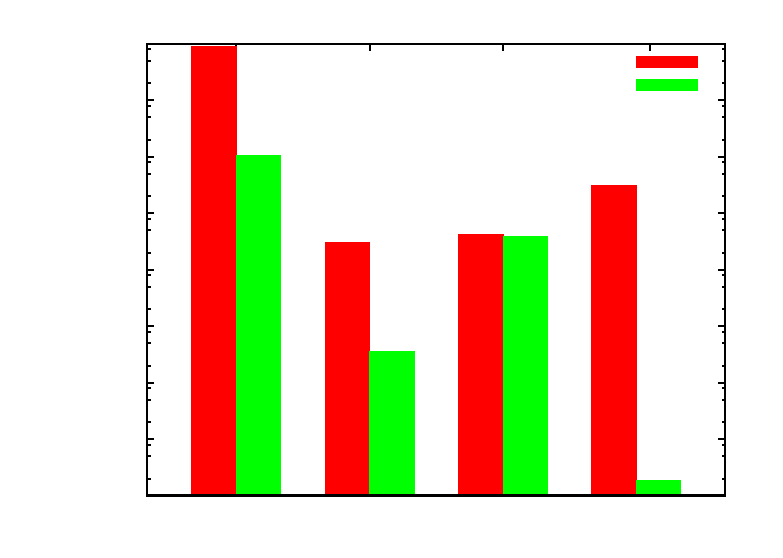
\includegraphics{rankPopcountDifference}}%
    \gplfronttext
  \end{picture}%
\endgroup

\end{figure}

\begin{figure}
\caption{Simple Binary Select vs. Binary Select using the Popcount instruction.}
\label{fig:selectPopcountDiff}
% GNUPLOT: LaTeX picture with Postscript
\begingroup
  \makeatletter
  \providecommand\color[2][]{%
    \GenericError{(gnuplot) \space\space\space\@spaces}{%
      Package color not loaded in conjunction with
      terminal option `colourtext'%
    }{See the gnuplot documentation for explanation.%
    }{Either use 'blacktext' in gnuplot or load the package
      color.sty in LaTeX.}%
    \renewcommand\color[2][]{}%
  }%
  \providecommand\includegraphics[2][]{%
    \GenericError{(gnuplot) \space\space\space\@spaces}{%
      Package graphicx or graphics not loaded%
    }{See the gnuplot documentation for explanation.%
    }{The gnuplot epslatex terminal needs graphicx.sty or graphics.sty.}%
    \renewcommand\includegraphics[2][]{}%
  }%
  \providecommand\rotatebox[2]{#2}%
  \@ifundefined{ifGPcolor}{%
    \newif\ifGPcolor
    \GPcolortrue
  }{}%
  \@ifundefined{ifGPblacktext}{%
    \newif\ifGPblacktext
    \GPblacktexttrue
  }{}%
  % define a \g@addto@macro without @ in the name:
  \let\gplgaddtomacro\g@addto@macro
  % define empty templates for all commands taking text:
  \gdef\gplbacktext{}%
  \gdef\gplfronttext{}%
  \makeatother
  \ifGPblacktext
    % no textcolor at all
    \def\colorrgb#1{}%
    \def\colorgray#1{}%
  \else
    % gray or color?
    \ifGPcolor
      \def\colorrgb#1{\color[rgb]{#1}}%
      \def\colorgray#1{\color[gray]{#1}}%
      \expandafter\def\csname LTw\endcsname{\color{white}}%
      \expandafter\def\csname LTb\endcsname{\color{black}}%
      \expandafter\def\csname LTa\endcsname{\color{black}}%
      \expandafter\def\csname LT0\endcsname{\color[rgb]{1,0,0}}%
      \expandafter\def\csname LT1\endcsname{\color[rgb]{0,1,0}}%
      \expandafter\def\csname LT2\endcsname{\color[rgb]{0,0,1}}%
      \expandafter\def\csname LT3\endcsname{\color[rgb]{1,0,1}}%
      \expandafter\def\csname LT4\endcsname{\color[rgb]{0,1,1}}%
      \expandafter\def\csname LT5\endcsname{\color[rgb]{1,1,0}}%
      \expandafter\def\csname LT6\endcsname{\color[rgb]{0,0,0}}%
      \expandafter\def\csname LT7\endcsname{\color[rgb]{1,0.3,0}}%
      \expandafter\def\csname LT8\endcsname{\color[rgb]{0.5,0.5,0.5}}%
    \else
      % gray
      \def\colorrgb#1{\color{black}}%
      \def\colorgray#1{\color[gray]{#1}}%
      \expandafter\def\csname LTw\endcsname{\color{white}}%
      \expandafter\def\csname LTb\endcsname{\color{black}}%
      \expandafter\def\csname LTa\endcsname{\color{black}}%
      \expandafter\def\csname LT0\endcsname{\color{black}}%
      \expandafter\def\csname LT1\endcsname{\color{black}}%
      \expandafter\def\csname LT2\endcsname{\color{black}}%
      \expandafter\def\csname LT3\endcsname{\color{black}}%
      \expandafter\def\csname LT4\endcsname{\color{black}}%
      \expandafter\def\csname LT5\endcsname{\color{black}}%
      \expandafter\def\csname LT6\endcsname{\color{black}}%
      \expandafter\def\csname LT7\endcsname{\color{black}}%
      \expandafter\def\csname LT8\endcsname{\color{black}}%
    \fi
  \fi
  \setlength{\unitlength}{0.0500bp}%
  \begin{picture}(7200.00,5040.00)%
    \gplgaddtomacro\gplbacktext{%
      \csname LTb\endcsname%
      \put(1122,440){\makebox(0,0)[r]{\strut{} 1000}}%
      \put(1122,982){\makebox(0,0)[r]{\strut{} 10000}}%
      \put(1122,1524){\makebox(0,0)[r]{\strut{} 100000}}%
      \put(1122,2066){\makebox(0,0)[r]{\strut{} 1e+06}}%
      \put(1122,2608){\makebox(0,0)[r]{\strut{} 1e+07}}%
      \put(1122,3149){\makebox(0,0)[r]{\strut{} 1e+08}}%
      \put(1122,3691){\makebox(0,0)[r]{\strut{} 1e+09}}%
      \put(1122,4233){\makebox(0,0)[r]{\strut{} 1e+10}}%
      \put(1122,4775){\makebox(0,0)[r]{\strut{} 1e+11}}%
      \put(2108,220){\makebox(0,0){\strut{}CPU Cycles}}%
      \put(3388,220){\makebox(0,0){\strut{}Wall Time}}%
      \put(4669,220){\makebox(0,0){\strut{}Cache Miss}}%
      \put(6077,220){\makebox(0,0){\strut{}Branch Mispr.}}%
    }%
    \gplgaddtomacro\gplfronttext{%
      \csname LTb\endcsname%
      \put(5816,4602){\makebox(0,0)[r]{\strut{}Simple Binary Rank }}%
      \csname LTb\endcsname%
      \put(5816,4382){\makebox(0,0)[r]{\strut{}Binary Rank using Popcount}}%
    }%
    \gplbacktext
    \put(0,0){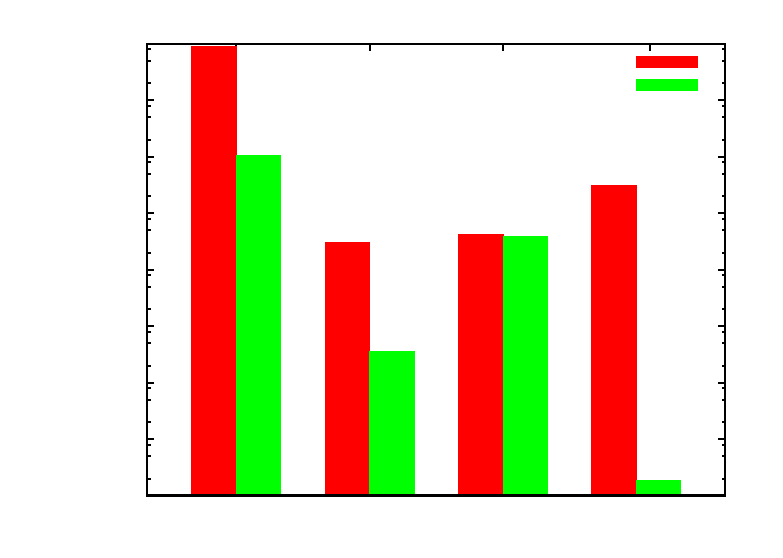
\includegraphics{rankPopcountDifference}}%
    \gplfronttext
  \end{picture}%
\endgroup

\end{figure}



[We then had the idea of skewing the tree to reduce branch mispredictions and cache-misses. but to reduce cache misses, we also need to control the memory layout... see following section]